\section{Architecture}

The following picture shows the core components and interfaces

\begin{figure}[h]
    \centering
    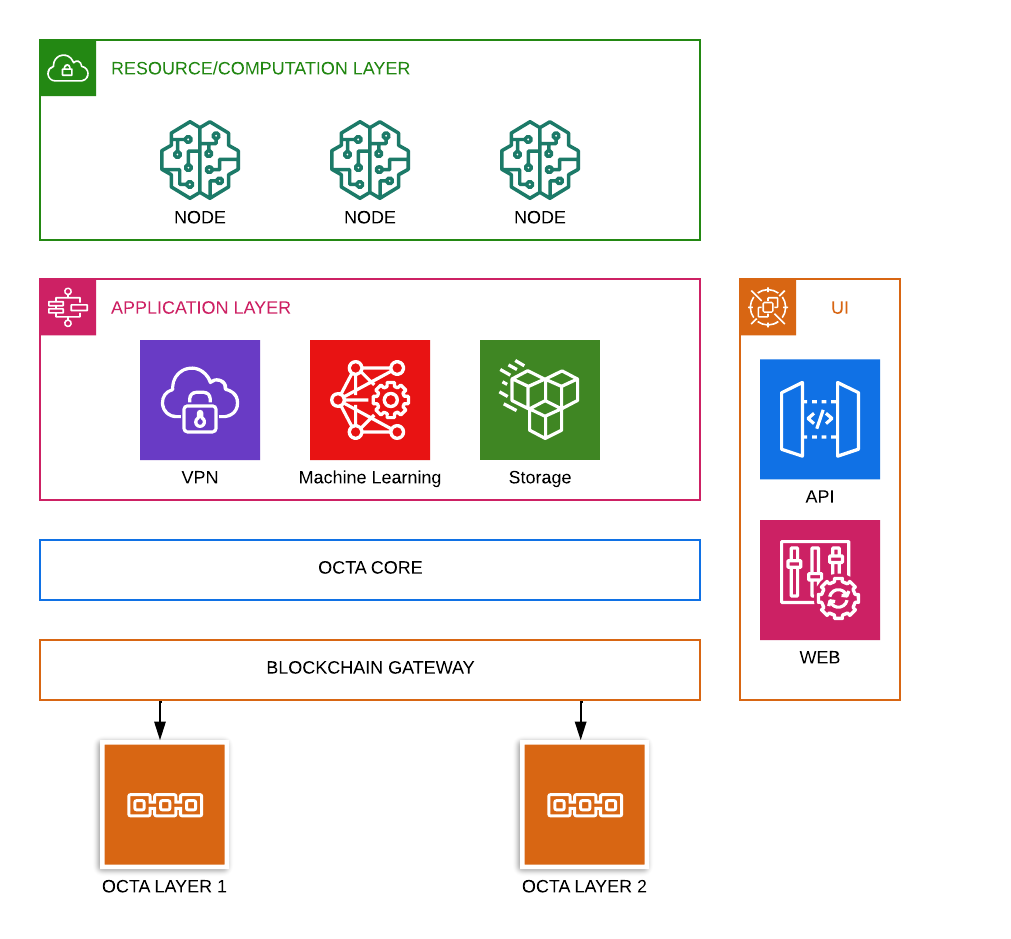
\includegraphics[width=\textwidth]{octa-arch}
    \caption{High Level Architecture}
\end{figure}

\subsection{Blockchain}
OctaSpace employs a multi-layered blockchain system to provide a secure and efficient platform for users.

At its core is a Layer 1 PoW blockchain, secured using the pirl 51\% guard technique, which provides robust protection against network attacks.
In addition, OctaSpace uses a Layer 2 PoA blockchain, based on validators, to speed up transactions for billing operations without compromising the security of the Layer 1 blockchain.

By using this Layer 2 PoA blockchain, OctaSpace can process a high volume of transactions quickly and efficiently
for billing operations such as charging users for the services they have used.

The platform's innovative blockchain architecture demonstrates its commitment to providing a secure and stable platform for its users, while ensuring fast and efficient billing transactions.
Overall, OctaSpace's blockchain infrastructure is a testament to its focus on security and efficiency, providing a reliable and scalable solution for distributed computing.

\newpage

\subsection{Layer 1 network}

\textbf{OctaSpace's Layer 1} network is Proof-of-Work (PoW\cite{pow}) blockchain used for frontend user financial operations using the native coin OCTA.

Network based on go-ethereum\cite{go-ethereum} codebase with the following specification:

\begin{itemize}
    \item Block time is 15 seconds
    \item Total supply is unlimited\footnote{Total supply will be reviewed after Mahasim fork}
    \item Block reward and halving implemented according to \hyperref[sec:mp]{Monenary policy}
    \item PirlGuard is used as protection mechanism from 51\% attack
    \item Transaction fee is 21 Gwei
\end{itemize}

To ensure a fair and transparent network without any premine or presale, OctaSpace designed its network with an equitable distribution of rewards. The genesis difficulty was set at 100Gh, preventing the instant allocation of rewards

\subsection{Layer 2 network}

OctaSpace employs a Layer 2 PoA network that serves as a side chain for the Layer 1 network.

This PoA network is used for internal transactions related to the node services and is supported by a set of validators.

The Layer 2 network is designed to handle high-frequency, high-usage operations with lightning-fast performance and seamless operation.
This translates to reduced operational costs, speedy transactions, and a massive boost in charging operations throughput for OctaSpace.

By utilizing this Layer 2 PoA network, OctaSpace can ensure fast and efficient processing of internal transactions, allowing for a smoother user experience and improved overall platform performance.


\subsection{Blockchain gateways}


OctaSpace Blockchain Gateways provide a unified API for the OCTA CORE layer to work with both blockchain networks.

The gateways' API is private and not accessible from outside the OctaSpace platform.

\subsection{OCTA CORE and Application Layer}

The OCTA CORE and Application Layer serves as the engine of the system, seamlessly handling all requests for compute rentals and providing an interface for creating services on top of resources provided by nodes.

It communicates with the nodes and user applications, making it effortless for users to access and use the resources.

Other core engine operations of the OCTA CORE and Application Layer include:

\begin{itemize}
    \item Communicating with nodes, monitoring and low-level interaction
    \item Handle requests for computing resources
    \item Provide interface for creating services on a top of resources provided by nodes
    \item Services usage charging and billing operations
    \item Provide API for automation or integration with third party systems
    \item Implementing fraud control
    \item Generating statistics and telemetry of system usage
\end{itemize}

\subsection{Resource Layer}
OCTA Chain is a powerful blockchain network, but the primary goal of the project is to provide practical applications and to bridge the gap between those who have computational resources and those who need them. This is where Octa nodes come in.

This layer consist of hardware(nodes) connected to the OctaSpace cloud.

These hardware nodes are connected to the OctaSpace cloud and form the foundation of our compute and services marketplace,
providing the necessary computational power to meet the demands of various tasks and services.

The nodes are equipped with a blend of CPUs, GPUs, memory, and disk space that allows them to handle distributed workloads with ease.
OctaSpace seamlessly connects these nodes together to deliver optimal performance and efficiency.

Machines with powerful GPUs can perform AI/ML tasks, while common machines can act as VPN gateways or provide disk storage for services like file sharing or host applications deployed by users.

\subsection{API and UI}

The following interfaces are available for interacting with the system:

\begin{itemize}
    \item Web applicaton with user-friendly interface accessible at \url{https://cube.octa.space}
    \item RESTful API
    \item An \textbf{octactl} command-line utility that provide user friendly interface to RESTful API
\end{itemize}
